\chapter{Teaching Your PI Controller to Behave (Part V)}
So far in this series, we have discussed how to distill the design of a cascaded velocity controller from a bunch of  seemingly uncorrelated PI coefficients down to a single system parameter; the \textit{damping factor} ($\delta$).  The damping factor represents the tradeoff between system stability and system bandwidth in a single parameter.  But how do you choose an appropriate damping factor value for your design, and what does it mean in terms of your system’s transient response?

To help answer these questions, let’s take a look at Figure \ref{fig:05_01}, which illustrates the \textit{open-loop} magnitude and phase response for a speed control system.  Note that all frequencies are scaled to the value of the velocity filter pole.  Assuming that the current controller's pole is very high with respect to this pole, the \textit{shape} of the curves won’t change, regardless of the velocity pole value.  In Figure \ref{fig:05_01}, the damping factor is swept from \num{70} to \num{1.5} in 8 discrete steps to show how it affects system response.  A $\delta$ value of \num{1.0} corresponds to the condition where the open-loop magnitude response has unity gain at the same frequency as the velocity filter's pole.  This scenario results in the velocity filter pole exactly cancelling out the zero which is creating all that nice phase lead we need to stabilize our system.  So we see that a $\delta$ value of \num{1.0} yields a system with zero phase margin, which of course is unstable.

\begin{figure}[H]
    \centering
    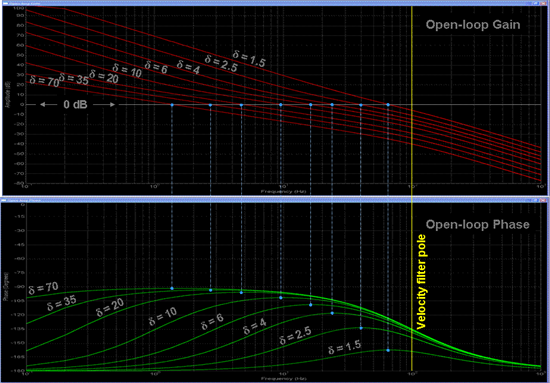
\includegraphics[width=1\linewidth]{05/01}
    \caption{Velocity Controller Open Loop Magnitude and Phase Response as a Function of $\delta$.}
    \label{fig:05_01}
\end{figure}

One of the goals of the damping factor is to achieve maximum stability for a given bandwidth.  This is confirmed in the plots above, which show that the phase margin always peaks to its maximum value at the unity gain frequency.  As the damping factor is increased, you eventually reach a point of diminishing returns for phase margin improvement as the signal phase shift approaches \qty{-90}{\degree}.  However, the \textit{gain} margin continues to improve as the damping factor is increased.

Figure \ref{fig:05_02} illustrates the \textit{closed-loop} magnitude response of the velocity loop with respect to the velocity filter pole as $\delta$ is swept from \num{70} to \num{1.5}.

\begin{figure}[H]
    \centering
    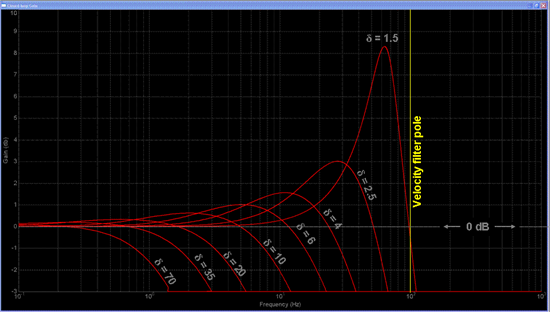
\includegraphics[width=1\linewidth]{05/02}
    \caption{Velocity Controller Closed Loop Bandwidth as a Function of $\delta$.}
    \label{fig:05_02}
\end{figure}

From figure \ref{fig:05_02} you can see how decreasing the damping factor increases the bandwidth of the velocity loop.  In fact, decreasing the damping factor from \num{70} to \num{1.5} increases the bandwidth by almost two orders of magnitude.  But as the damping factor approaches unity, the complex poles in the velocity loop approach the $j\omega$ axis, resulting in pronounced peaking of the gain response.  This peaking effect is usually undesirable, as it results in excessive underdamped ringing of the step response.  You can better see this in figure \ref{fig:05_03}, which shows the normalized step response of the system for various values of damping factor.  Values below 2 are usually unacceptable due to the large amount of overshoot they produce.  At the other end of the scale, values much above 35 produce extremely long rise and settling times.  Your design target window will usually be somewhere in-between these two values.

\begin{figure}[H]
    \centering
    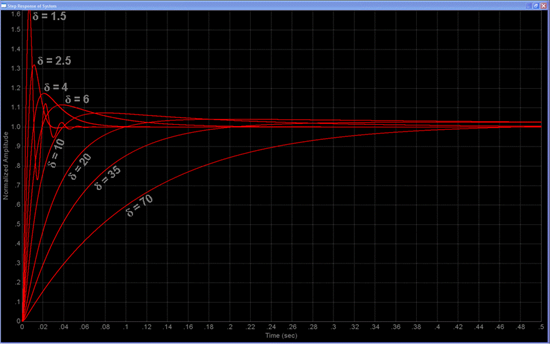
\includegraphics[width=1\linewidth]{05/03}
    \caption{Step Response of Velocity Controller as a Function of $\delta$.}
    \label{fig:05_03}
\end{figure}

What happens if you pick a damping factor based on a desired \textit{shape} for your step response, but the response \textit{time} is too long?  Well, assuming you have the design flexibility to do so, your best recourse might be to increase the velocity filter pole.  In figures \ref{fig:05_01} and \ref{fig:05_02}, all frequencies are scaled to this pole value, which means that if you change it, all other frequencies will change proportionally.  So if you double the value of the velocity filter pole in figures \ref{fig:05_01} and \ref{fig:05_02}, you will half the time axis in figure \ref{fig:05_03}.

But what if you \textit{don’t} have this flexibility?  Unfortunately, you will be forced to choose between response time and overshoot.  In other words, you can solve one problem or the other, but not both at the same time.  It’s kind of like a water balloon.  You can squeeze it down in one spot, but it will pop up somewhere else.  I know\dots it’s not fair.  But that’s the way life is sometimes.

So far we have discussed how to set three of the four PI coefficients in a velocity control loop.  But there is still one left\dots $K_a$.  Recall that $K_a$ sets the bandwidth of the current controller.  In many respects, $K_a$ is the hardest one to set since its effect on system performance is more subjective than the other three.  In my next blog, let’s take a closer look at $K_a$, its impact on system performance, and hopefully gain some insight into how to set it correctly.  In the meantime\dots

Keep Those Motors Spinning,\\

\includegraphics[width=0.2\linewidth]{01/04_dave}
\vfill
\textit{Mar 23 2013 11:13 AM}